\documentclass[10pt]{article}

\usepackage[a4paper,margin=0.75in]{geometry}
\usepackage[T1]{fontenc}
\usepackage[utf8]{inputenc}
\usepackage{lmodern}
\usepackage{microtype}
\usepackage{amsmath,amssymb,mathtools}
\usepackage{booktabs,multirow}
\usepackage{siunitx}
\usepackage{graphicx}
\usepackage{tikz}
\usetikzlibrary{arrows.meta,positioning,shapes.geometric,fit}
\usepackage{algorithm}
\usepackage{algpseudocode}
\usepackage{enumitem}
\usepackage{xcolor}
\usepackage{hyperref}
\usepackage[nameinlink,capitalise]{cleveref}
\usepackage{natbib}
\usepackage{fancyhdr}
\usepackage{titlesec}
\usepackage{caption}

\definecolor{accent}{HTML}{285D50}
\definecolor{dark}{HTML}{18302A}
\definecolor{soft}{HTML}{EEF3F0}
\definecolor{muted}{HTML}{5B6662}

\hypersetup{
  colorlinks=true,
  linkcolor=accent,
  citecolor=accent,
  urlcolor=accent,
  pdfauthor={Rehema Mwawado},
  pdftitle={Scientific LaTeX Technical Writing Sample}
}

\pagestyle{fancy}
\fancyhf{}
\lhead{\small Scientific LaTeX Technical Writing Sample}
\rhead{\small Rehema Mwawado}
\cfoot{\thepage}
\renewcommand{\headrulewidth}{0.4pt}

\titleformat{\section}{\large\bfseries\color{dark}}{\thesection.}{0.55em}{}
\titleformat{\subsection}{\normalsize\bfseries\color{dark}}{\thesubsection}{0.5em}{}
\captionsetup{font=small,labelfont=bf}
\setlist[itemize]{leftmargin=1.4em,itemsep=2pt,topsep=4pt}
\setlength{\parindent}{0pt}
\setlength{\parskip}{5pt}
\sisetup{detect-all}

\newcommand{\R}{\mathbb{R}}
\newcommand{\E}{\mathbb{E}}
\newcommand{\loss}{\mathcal{L}}
\newcommand{\dataset}{\mathcal{D}}

\begin{document}

\begin{center}
{\small\bfseries\color{accent} PORTFOLIO SAMPLE}\\[5pt]
{\LARGE\bfseries Scientific LaTeX Technical Writing Sample}\\[7pt]
{\large Quality-Aware Federated Regression at the Edge}\\[8pt]
{\normalsize Rehema Mwawado}\\[3pt]
{\small Scientific writing \textbullet\ LaTeX/Overleaf \textbullet\ Mathematical typesetting \textbullet\ Research communication}
\end{center}

\vspace{5pt}
\noindent\colorbox{soft}{\parbox{0.965\linewidth}{\small
\textbf{Purpose.} This document is an original, non-confidential portfolio demonstration. It is designed to show scientific writing and LaTeX skills---including equations, notation, cross-references, algorithms, tables, figures, citations, and bibliography management---rather than to report a new empirical study.
}}

\section{Technical Context}

Federated learning (FL) enables multiple clients to optimize a shared model without pooling their raw data at a central server. In the canonical formulation, each client performs local optimization and communicates model updates for server-side aggregation \citep{mcmahan2017communication}. This paradigm is useful when data are distributed across devices, institutions, or sensing locations and when communication or privacy constraints make centralized training undesirable \citep{kairouz2021advances}.

Edge deployments introduce an additional challenge: not all client observations are equally informative. Measurements close to known sensor limits, temporary communication failures, or sparsely sampled periods may be less reliable than well-supported observations. A quality-aware objective can therefore be used to moderate the contribution of uncertain samples while retaining the decentralized training structure.

This short example develops a compact regression formulation. The technical goal is intentionally simple: predict a continuous target $y\in\R$ from a feature vector $\mathbf{x}\in\R^d$ while accounting for per-sample confidence. The emphasis is on clear scientific exposition and reproducible mathematical notation.

\subsection{Problem Definition and Notation}

Assume $K$ edge clients. Client $k$ owns a local dataset
\begin{equation}
\dataset_k = \left\{\left(\mathbf{x}_{k,i},y_{k,i},q_{k,i}\right)\right\}_{i=1}^{n_k},
\label{eq:dataset}
\end{equation}
where $q_{k,i}\in[0,1]$ is a quality score and $n_k$ is the number of local samples. Let $f_{\boldsymbol{\theta}}(\mathbf{x})$ denote a regression model parameterized by $\boldsymbol{\theta}$.

For a single sample, the weighted squared-error loss is
\begin{equation}
\ell_{k,i}(\boldsymbol{\theta})
= q_{k,i}\left(y_{k,i}-f_{\boldsymbol{\theta}}(\mathbf{x}_{k,i})\right)^2.
\label{eq:sample-loss}
\end{equation}
The normalized local objective becomes
\begin{equation}
\loss_k(\boldsymbol{\theta})
= \frac{1}{\sum_{i=1}^{n_k}q_{k,i}+\varepsilon}
\sum_{i=1}^{n_k}\ell_{k,i}(\boldsymbol{\theta}),
\label{eq:local-objective}
\end{equation}
where $\varepsilon>0$ avoids division by zero. The global objective is
\begin{align}
\min_{\boldsymbol{\theta}}\quad
\loss(\boldsymbol{\theta})
&= \sum_{k=1}^{K}\alpha_k\loss_k(\boldsymbol{\theta}), \\
\alpha_k
&= \frac{n_k}{\sum_{j=1}^{K} n_j}.
\label{eq:global-objective}
\end{align}
Equations~\eqref{eq:local-objective}--\eqref{eq:global-objective} separate two weighting mechanisms: $q_{k,i}$ controls within-client sample influence, whereas $\alpha_k$ controls the client contribution during aggregation.

\section{System Workflow}

The workflow in \cref{fig:workflow} separates sensing, local optimization, and server aggregation. Raw observations remain at the client. Only model parameters or parameter updates are transmitted.

\begin{figure}[htbp]
\centering
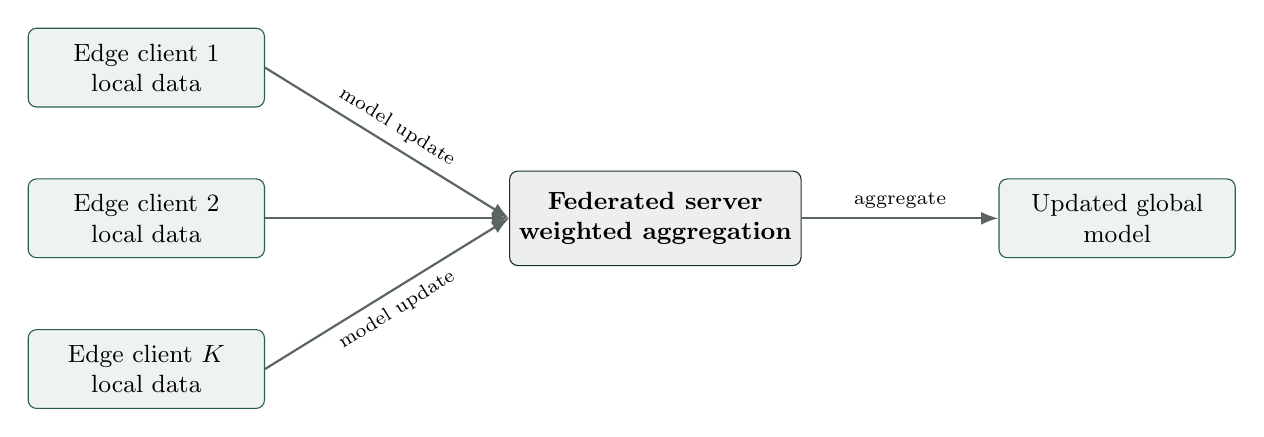
\begin{tikzpicture}[
  node distance=9mm and 13mm,
  box/.style={draw=accent, rounded corners=3pt, fill=soft, minimum width=30mm, minimum height=10mm, align=center, font=\small},
  server/.style={draw=dark, rounded corners=3pt, fill=dark!8, minimum width=36mm, minimum height=12mm, align=center, font=\small\bfseries},
  arrow/.style={-{Latex[length=2.2mm]}, thick, draw=muted}
]
\node[box] (c1) {Edge client 1\\local data};
\node[box, below=of c1] (c2) {Edge client 2\\local data};
\node[box, below=of c2] (c3) {Edge client $K$\\local data};
\node[server, right=31mm of c2] (srv) {Federated server\\weighted aggregation};
\node[box, right=25mm of srv] (model) {Updated global\\model};

\draw[arrow] (c1.east) -- node[above,sloped,font=\scriptsize]{model update} (srv.west);
\draw[arrow] (c2.east) -- (srv.west);
\draw[arrow] (c3.east) -- node[below,sloped,font=\scriptsize]{model update} (srv.west);
\draw[arrow] (srv) -- node[above,font=\scriptsize]{aggregate} (model);
\end{tikzpicture}
\caption{Illustrative federated regression workflow. Client data remain local; only model information is exchanged.}
\label{fig:workflow}
\end{figure}

At round $t$, the server broadcasts $\boldsymbol{\theta}^{(t)}$. Each selected client performs $E$ local epochs and returns updated parameters $\boldsymbol{\theta}^{(t+1)}_k$. A FedAvg-style aggregation step \citep{mcmahan2017communication} is then
\begin{equation}
\boldsymbol{\theta}^{(t+1)}
= \sum_{k\in\mathcal{S}_t}
\frac{n_k}{\sum_{j\in\mathcal{S}_t}n_j}
\boldsymbol{\theta}^{(t+1)}_k,
\label{eq:aggregation}
\end{equation}
where $\mathcal{S}_t$ denotes the clients participating in round $t$.

\subsection{Algorithmic Description}

\Cref{alg:qafl} gives a concise training procedure. The pseudocode makes the data flow explicit and distinguishes local sample weighting from server-side client aggregation.

\begin{algorithm}[htbp]
\caption{Quality-Aware Federated Regression}
\label{alg:qafl}
\begin{algorithmic}[1]
\Require Clients $\{1,\ldots,K\}$, rounds $T$, local epochs $E$, learning rate $\eta$
\State Initialize global parameters $\boldsymbol{\theta}^{(0)}$
\For{$t=0,1,\ldots,T-1$}
    \State Server selects participating clients $\mathcal{S}_t$
    \ForAll{$k\in\mathcal{S}_t$ \textbf{in parallel}}
        \State Set $\boldsymbol{\theta}_k \gets \boldsymbol{\theta}^{(t)}$
        \For{$e=1,\ldots,E$}
            \State Compute $\nabla\loss_k(\boldsymbol{\theta}_k)$ using \cref{eq:local-objective}
            \State $\boldsymbol{\theta}_k \gets \boldsymbol{\theta}_k - \eta\nabla\loss_k(\boldsymbol{\theta}_k)$
        \EndFor
        \State Return $\boldsymbol{\theta}_k$ and $n_k$ to server
    \EndFor
    \State Aggregate client models using \cref{eq:aggregation}
\EndFor
\State \Return final global model $\boldsymbol{\theta}^{(T)}$
\end{algorithmic}
\end{algorithm}

\section{Evaluation and Reporting}

A scientific report should distinguish predictive performance from deployment cost. For regression, root mean squared error (RMSE), mean absolute error (MAE), and coefficient of determination ($R^2$) are common complementary metrics. RMSE is defined as
\begin{equation}
\operatorname{RMSE}
= \sqrt{\frac{1}{N}\sum_{i=1}^{N}\left(y_i-\hat{y}_i\right)^2}.
\label{eq:rmse}
\end{equation}
Communication can be summarized using transmitted bytes per round, whereas edge feasibility can include peak memory, local training time, and model size.

\begin{table}[htbp]
\centering
\caption{Illustrative reporting structure for a federated regression experiment. Values are synthetic and included only to demonstrate scientific table formatting.}
\label{tab:results}
\small
\begin{tabular}{lrrrr}
\toprule
Method & RMSE & MAE & $R^2$ & Comm. (MB) \\
\midrule
Centralized reference & 0.082 & 0.061 & 0.88 & -- \\
FedAvg & 0.091 & 0.068 & 0.85 & 14.2 \\
Quality-aware FL & \textbf{0.086} & \textbf{0.064} & \textbf{0.87} & 14.2 \\
Local only & 0.108 & 0.079 & 0.78 & 0.0 \\
\bottomrule
\end{tabular}
\end{table}

The example in \cref{tab:results} demonstrates a reporting convention rather than a research result. In a real study, numerical comparisons should be accompanied by uncertainty estimates, clearly defined train/validation/test partitions, and a statement of whether hyperparameters were tuned using validation data only. When multiple clients are evaluated, reporting both aggregate metrics and the distribution across clients helps expose performance heterogeneity.

\subsection{Reproducibility Checklist}

A compact reproducibility section can make technical work easier to audit. At minimum, a manuscript should specify:
\begin{itemize}
    \item the data partitioning strategy and any exclusion criteria;
    \item preprocessing, normalization, and missing-data handling;
    \item model architecture, optimizer, learning rate, batch size, and random seeds;
    \item FL participation rate, number of rounds, and local epochs;
    \item metric definitions and the unit of aggregation; and
    \item software versions, hardware, and availability of code or configuration files.
\end{itemize}

These details are especially important in FL because client partitioning and local training choices can materially alter the optimization problem \citep{li2020federated}.

\section{Technical Writing Notes}

This sample intentionally demonstrates several document-production capabilities in one short artifact:
\begin{itemize}
    \item consistent mathematical notation across \cref{eq:dataset,eq:global-objective,eq:aggregation};
    \item automatic numbering and cross-referencing for equations, figures, tables, sections, and algorithms;
    \item a vector workflow diagram created directly in TikZ;
    \item a professional table using \texttt{booktabs};
    \item structured pseudocode using \texttt{algorithm} and \texttt{algpseudocode};
    \item bibliography management using BibTeX-compatible citations; and
    \item concise technical prose that distinguishes assumptions, definitions, procedures, and evidence.
\end{itemize}

The same workflow can be adapted to publisher-specific templates such as IEEE, Springer, or Elsevier while preserving consistent notation, references, figures, and document structure.

\section{Conclusion}

This portfolio document presents a compact example of scientific LaTeX preparation for a machine-learning topic. The emphasis is not on proposing a novel algorithm, but on demonstrating how technical content can be organized into a coherent, publication-style document with traceable definitions, equations, algorithms, figures, tables, and references.

\section*{Document Production Details}
The public source package accompanying this PDF contains the complete \texttt{.tex} file and a separate \texttt{references.bib} database. The PDF is intentionally self-contained for straightforward compilation on a standard TeX installation; the bibliography database is provided to demonstrate a reusable BibTeX workflow for publisher templates. Core packages used in this sample include \texttt{amsmath}, \texttt{cleveref}, \texttt{booktabs}, \texttt{algorithmicx}, and \texttt{TikZ}.

A minimal reproducible build consists of two LaTeX passes:
\begin{center}
\small\texttt{pdflatex scientific-latex-sample.tex}\quad $\rightarrow$ \quad
\texttt{pdflatex scientific-latex-sample.tex}
\end{center}

\begin{thebibliography}{9}

\bibitem[McMahan et~al.(2017)]{mcmahan2017communication}
H.~B. McMahan, E. Moore, D. Ramage, S. Hampson, and B. Ag\"uera y Arcas,
``Communication-efficient learning of deep networks from decentralized data,''
in \emph{Proc. 20th Int. Conf. Artificial Intelligence and Statistics}, 2017,
pp. 1273--1282.

\bibitem[Kairouz et~al.(2021)]{kairouz2021advances}
P. Kairouz, H.~B. McMahan, B. Avent, et~al.,
``Advances and open problems in federated learning,''
\emph{Foundations and Trends in Machine Learning}, vol. 14, nos. 1--2,
pp. 1--210, 2021.

\bibitem[Li et~al.(2020)]{li2020federated}
T. Li, A.~K. Sahu, M. Zaheer, M. Sanjabi, A. Talwalkar, and V. Smith,
``Federated optimization in heterogeneous networks,''
\emph{Proceedings of Machine Learning and Systems}, vol. 2,
pp. 429--450, 2020.

\end{thebibliography}

\end{document}
